% Copyright © 2015-2016 Martin Ueding <dev@martin-ueding.de>
%
\documentclass[english, fleqn]{beamer}

\usetheme{Malmoe}
%\usetheme{Dresden}
%\usetheme{Marburg}

\usepackage[bibatend, beamer]{../../header}
\usepackage{adjustbox}
\usepackage{transparent}

\renewcommand\iup{\text i}
\renewcommand\eup{\text e}

\graphicspath{{./}{../Figures/}}

\title{K225 Positron lifetime in metals and insulators}
\subtitle{Advanced Lab Course -- Universität Bonn}
\author{%
    Martin Ueding
    \and
    Lino Lemmer
}
\date{Experiment: \daterange{2016-03-24}{2016-03-25} \\ Talk: 2016-04-29}

\newcommand\transition[2]{%
    {
        \setbeamertemplate{background canvas}{%
            \includegraphics[height=\paperheight]{#2}
        }
        \begin{frame}[plain]
            \centering
            \transparent{0.8}
            \colorbox{white}{%
                \marginbox{1ex}{%
                    \begin{huge}
                        #1
                    \end{huge}
                }
            }
        \end{frame}
    }
}

\newcommand\oscillatorSize{0.7}

\begin{document}

\begin{frame}
    \titlepage
\end{frame}

\section{Introduction}

\begin{frame}
    \frametitle{Aims of the experiment}
    \begin{itemize}
        \item 
            Measurement of temperature dependence of the positron lifetimes in indium
        \item
            Estimation of vacancy formation enthalpy
        \item
            Measurement of positronium lifetimes in acrylic glass
    \end{itemize}
\end{frame}

\section{Theory}

\subsection{Positrons}

\begin{frame}
    \frametitle{Positron source}
    \begin{columns}[c]
        \column{.5\textwidth}
        \begin{itemize}
            \item 
                ${}^{22}\text{Na}$ as source
            \item
                $\betaup^+$-decay into ${}^{22}\text{Ne}$
            \item
                Lifetime of excited Ne: \SI{3}{\pico\second} \\
                $\Rightarrow$ \SI{1276.4}{\kilo\electronvolt} is starting line
        \end{itemize}
        \column{.5\textwidth}
        \centering
        \includegraphics{beamer-na22}
    \end{columns}
\end{frame}

\begin{frame}
    \frametitle{Positron creation}
    \begin{columns}[c]
        \column{.5\textwidth}
        \begin{itemize}
            \item
                Convertion of up-quark in down-quark
            \item
                Creation of $\mathrm W^+$ boson
            \item
                Decay into $\mathrm e^+$ and $\nuup_\mathrm{e}$
        \end{itemize}
        \column{.5\textwidth}
        \centering
        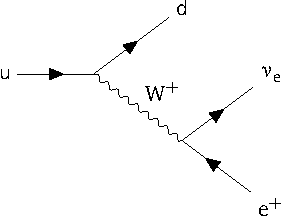
\includegraphics{beamer-beta}
    \end{columns}
\end{frame}

\begin{frame}
    \frametitle{Decay modes of positrons}

    \begin{columns}[T]
        \begin{column}{.5\textwidth}
            Spins antiparallel\\
            \vspace{1cm}
            \centering
            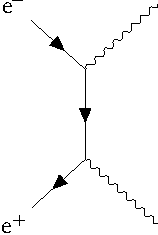
\includegraphics{beamer-two-photon}
        \end{column}
        \begin{column}{.5\textwidth}
            Spins parallel\\
            \centering
            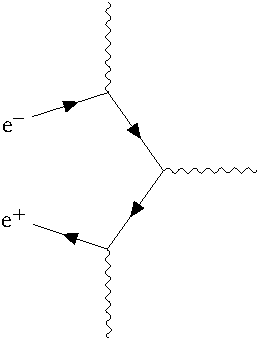
\includegraphics{beamer-three-photon}
        \end{column}
    \end{columns}
\end{frame}

\begin{frame}
    \frametitle{Positronium}
    \begin{itemize}
        \item
            hydrogen-like metastable bound state of electron and positron
        \item
            two possible configurations:
            \begin{itemize}
                \item
                    para-positronium: spins antiparallel
                \item
                    ortho-positronium: spins parallel
            \end{itemize}
        \item
            lifetime depends on if it is free or trapped and on configuration 
        \item
            pick-off process reduces ortho-positronium's lifetime in presence of matter
    \end{itemize}
\end{frame}

\subsection{Lattice defects}

\begin{frame}
    \frametitle{}
\end{frame}

\subsection{Detector and electronics}

\begin{frame}
    \frametitle{\textsc{Lyso} scintillator}
    Operation of a scintillator known:
    \pause
    \begin{itemize}
        \item 
            Ionizing radiation loses all its energy by exciting scintillator material
        \item
            Excited atoms or molecules go back to ground state via some other states
        \item
            Results in light glowing of the material
        \item
            Intensity proportional to particle's energy
    \end{itemize}
    \textsc{Lyso} scintillator is radioactive itself\\
    $\Rightarrow$ intrinsic energy calibration
\end{frame}

\begin{frame}
    \frametitle{\textsc{Lyso} scintillator}
    \centering
    \includegraphics{beamer-scheme-176Lu}
\end{frame}

\begin{frame}
    \frametitle{Photomultiplier}
    \includegraphics{beamer-photomultiplier}
    \pause
    Different signal types depending on where signal is taken:
    \begin{itemize}
        \item 
            Anode: Rising quickly, possibly saturated $\Rightarrow$ fast signal
        \item
            Dinode: Rising slower, energy proportional $\Rightarrow$ slow signal
    \end{itemize}
\end{frame}

\begin{frame}
    \frametitle{Electronic components}
    \begin{description}
    \item[\textsc{sca}]
        “Single channel analizer”. Takes analog signal, gives digital pulse if amplitude lies in certain interval (“\textsc{sca} window”)
    \item[\textsc{cfd}]
        “Constant fraction discriminator”. Takes analog signal, gives digital pulse if amplitude lies above a certain value when a defined fraction of the amplitude is reached
    \item[\textsc{tac}]
        “Time-amplitude converter”. Takes two digital pulses, gives a signal with amplitude proportional to the time between the two pulses
    \item[\textsc{mca}]
        “Multi channel analizer”. Creates histogram of incoming analog pulse heights
    \end{description}
\end{frame}

\begin{frame}
    \frametitle{Fast-slow-coincidence circuit}
    \centering
    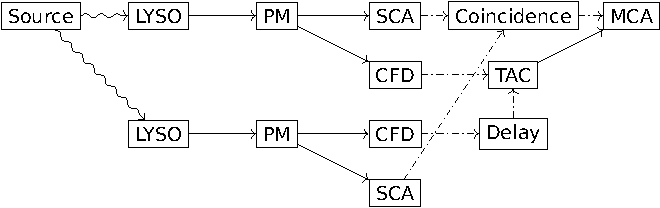
\includegraphics{beamer-fast-slow}
\end{frame}

\subsection{Bootstrap}

\transition{Bootstrap}{boots-3}

\begin{frame}
    \frametitle{The usual way}
    \framesubtitle{Some data}
    \centering
    \includegraphics{beamer-bootstrap-raw}
\end{frame}

\begin{frame}
    \frametitle{The usual way}
    \framesubtitle{A linear fit}
    \centering
    \includegraphics{beamer-bootstrap-fit}
\end{frame}

\begin{frame}
    \frametitle{The usual way}
    \framesubtitle{Fit parameter error estimation}

    \begin{alertblock}{Problem}
        What are the errors on the two fit parameters?
    \end{alertblock}

    \pause

    \begin{block}{Common solutions}
        \begin{itemize}
            \item
                Perform linear regression only
            \item
                Use diagonal of covariance matrix
            \item
                Attempt Gaussian error propagation
        \end{itemize}
    \end{block}

    \pause

    None of them are particularly good!
\end{frame}


\begin{frame}
    \frametitle{Resampling}
    \framesubtitle{Idea}

    \begin{block}{Realization}
            Given errors imply a distribution. Error is standard deviation of a
            normal distribution.
    \end{block}

    \pause

    \begin{block}{Method}
        \begin{enumerate}
            \item Draw samples from implied normal distribution
            \item Perform analysis with re-sampled data
            \item Look at distribution of results
        \end{enumerate}
    \end{block}
\end{frame}

\begin{frame}
    \frametitle{Resampling}
    \framesubtitle{Original data}
    \centering
    \includegraphics{beamer-bootstrap-raw}
\end{frame}

\begin{frame}
    \frametitle{Resampling}
    \framesubtitle{Resample each point}
    \centering
    \includegraphics{beamer-bootstrap-resample-1.pdf}
\end{frame}

\begin{frame}
    \frametitle{Resampling}
    \framesubtitle{Perform a single fit}
    \centering
    \includegraphics{beamer-bootstrap-resample-2.pdf}
\end{frame}

\begin{frame}
    \frametitle{Resampling}
    \framesubtitle{Add more samples}
    \centering
    \includegraphics{beamer-bootstrap-resample-3.pdf}
\end{frame}

\begin{frame}
    \frametitle{Resampling}
    \framesubtitle{Perform another fit}
    \centering
    \includegraphics{beamer-bootstrap-resample-4.pdf}
\end{frame}

\begin{frame}
    \frametitle{Resampling}
    \framesubtitle{More samples and fit}
    \centering
    \includegraphics{beamer-bootstrap-resample-5.pdf}
\end{frame}

\begin{frame}
    \frametitle{Resampling}
    \framesubtitle{More samples and fit}
    \centering
    \includegraphics{beamer-bootstrap-resample-6.pdf}
\end{frame}

\begin{frame}
    \frametitle{Resampling}
    \framesubtitle{Lots of fits}
    \centering
    \includegraphics{beamer-bootstrap-resample-7.pdf}
\end{frame}

\begin{frame}
    \frametitle{Resampling}
    \framesubtitle{Band of fits}
    \centering
    \includegraphics{beamer-bootstrap-band}
\end{frame}

\begin{frame}
    Control over statistical fluctuations.

    \pause

    \alert{What about outliers?}

    \pause

    \begin{block}{Jackknife method}
        \begin{itemize}
            \item Remove one element
            \item Perform analysis
            \item Repeat with all points
        \end{itemize}
    \end{block}
\end{frame}

\begin{frame}
    \frametitle{Jackknife}
    \centering
    \includegraphics{beamer-jackknife-resample-1.pdf}
\end{frame}

\begin{frame}
    \frametitle{Jackknife}
    \centering
    \includegraphics{beamer-jackknife-resample-2.pdf}
\end{frame}

\begin{frame}
    \frametitle{Jackknife}
    \centering
    \includegraphics{beamer-jackknife-resample-3.pdf}
\end{frame}

\begin{frame}
    \frametitle{Jackknife}
    \centering
    \includegraphics{beamer-jackknife-resample-4.pdf}
\end{frame}

\begin{frame}
    \frametitle{Jackknife}
    \framesubtitle{Band of fits}
    \centering
    \includegraphics{beamer-jackknife-band}
\end{frame}

\begin{frame}
    \frametitle{Resampling and Jackknife}

    Both methods can be combined!
\end{frame}

\begin{frame}
    \frametitle{Resampling and Jackknife}
    \framesubtitle{Band of fits}
    \centering
    \includegraphics{beamer-combined-band}
\end{frame}

\begin{frame}
    \frametitle{Resampling and Jackknife}
    \framesubtitle{Band of fits}
    \centering
    \includegraphics{beamer-combined-band2}
\end{frame}

\begin{frame}
    \frametitle{Resampling and Jackknife}
    \framesubtitle{Comparison of methods}
    {
        \centering
        \begin{tabular}{lSS}
            \toprule
            {Method}
            & {$a$}
            & {$b$}
            \\
            \midrule
            \texttt{sqrt(pconv.diagonal())} & << ' & '.join(pconv_example_popt) >> \\
            Resampling & << ' & '.join(bootstrap_example_popt) >> \\
            Jackknife & << ' & '.join(jackknife_example_popt) >> \\
            Combined & << ' & '.join(combined_example_popt) >> \\
            \bottomrule
        \end{tabular}
    }

    \pause

    Data is generated from $y(x) = 1 \cdot x + 0$.

    \pause

    Standard method underestimates the error.

\end{frame}

\begin{frame}
    \frametitle{Resampling and Jackknife}
    \framesubtitle{Outlook}

    Further possible improvements:

    \begin{itemize}
        \item Use quantiles for assymetric error
        \item $\chi^2$ weighted histograms
    \end{itemize}

    \pause

    Not used in our analysis
\end{frame}

\section{Conduction}

\transition{Conduction}{rack-and-detector}

\subsection{Slow circuit setup}

\begin{frame}

    \centering
    \includegraphics{beamer-lyso-li}
\end{frame}

\begin{frame}

    \centering
    \includegraphics{beamer-lyso-re}
\end{frame}

\begin{frame}

    \centering
    \includegraphics{beamer-na-li}
\end{frame}

\begin{frame}

    \centering
    \includegraphics{beamer-na-re}
\end{frame}

\begin{frame}
    \frametitle{SCA and coincidence on \SI{511}{\kilo\electronvolt}}

    \centering
    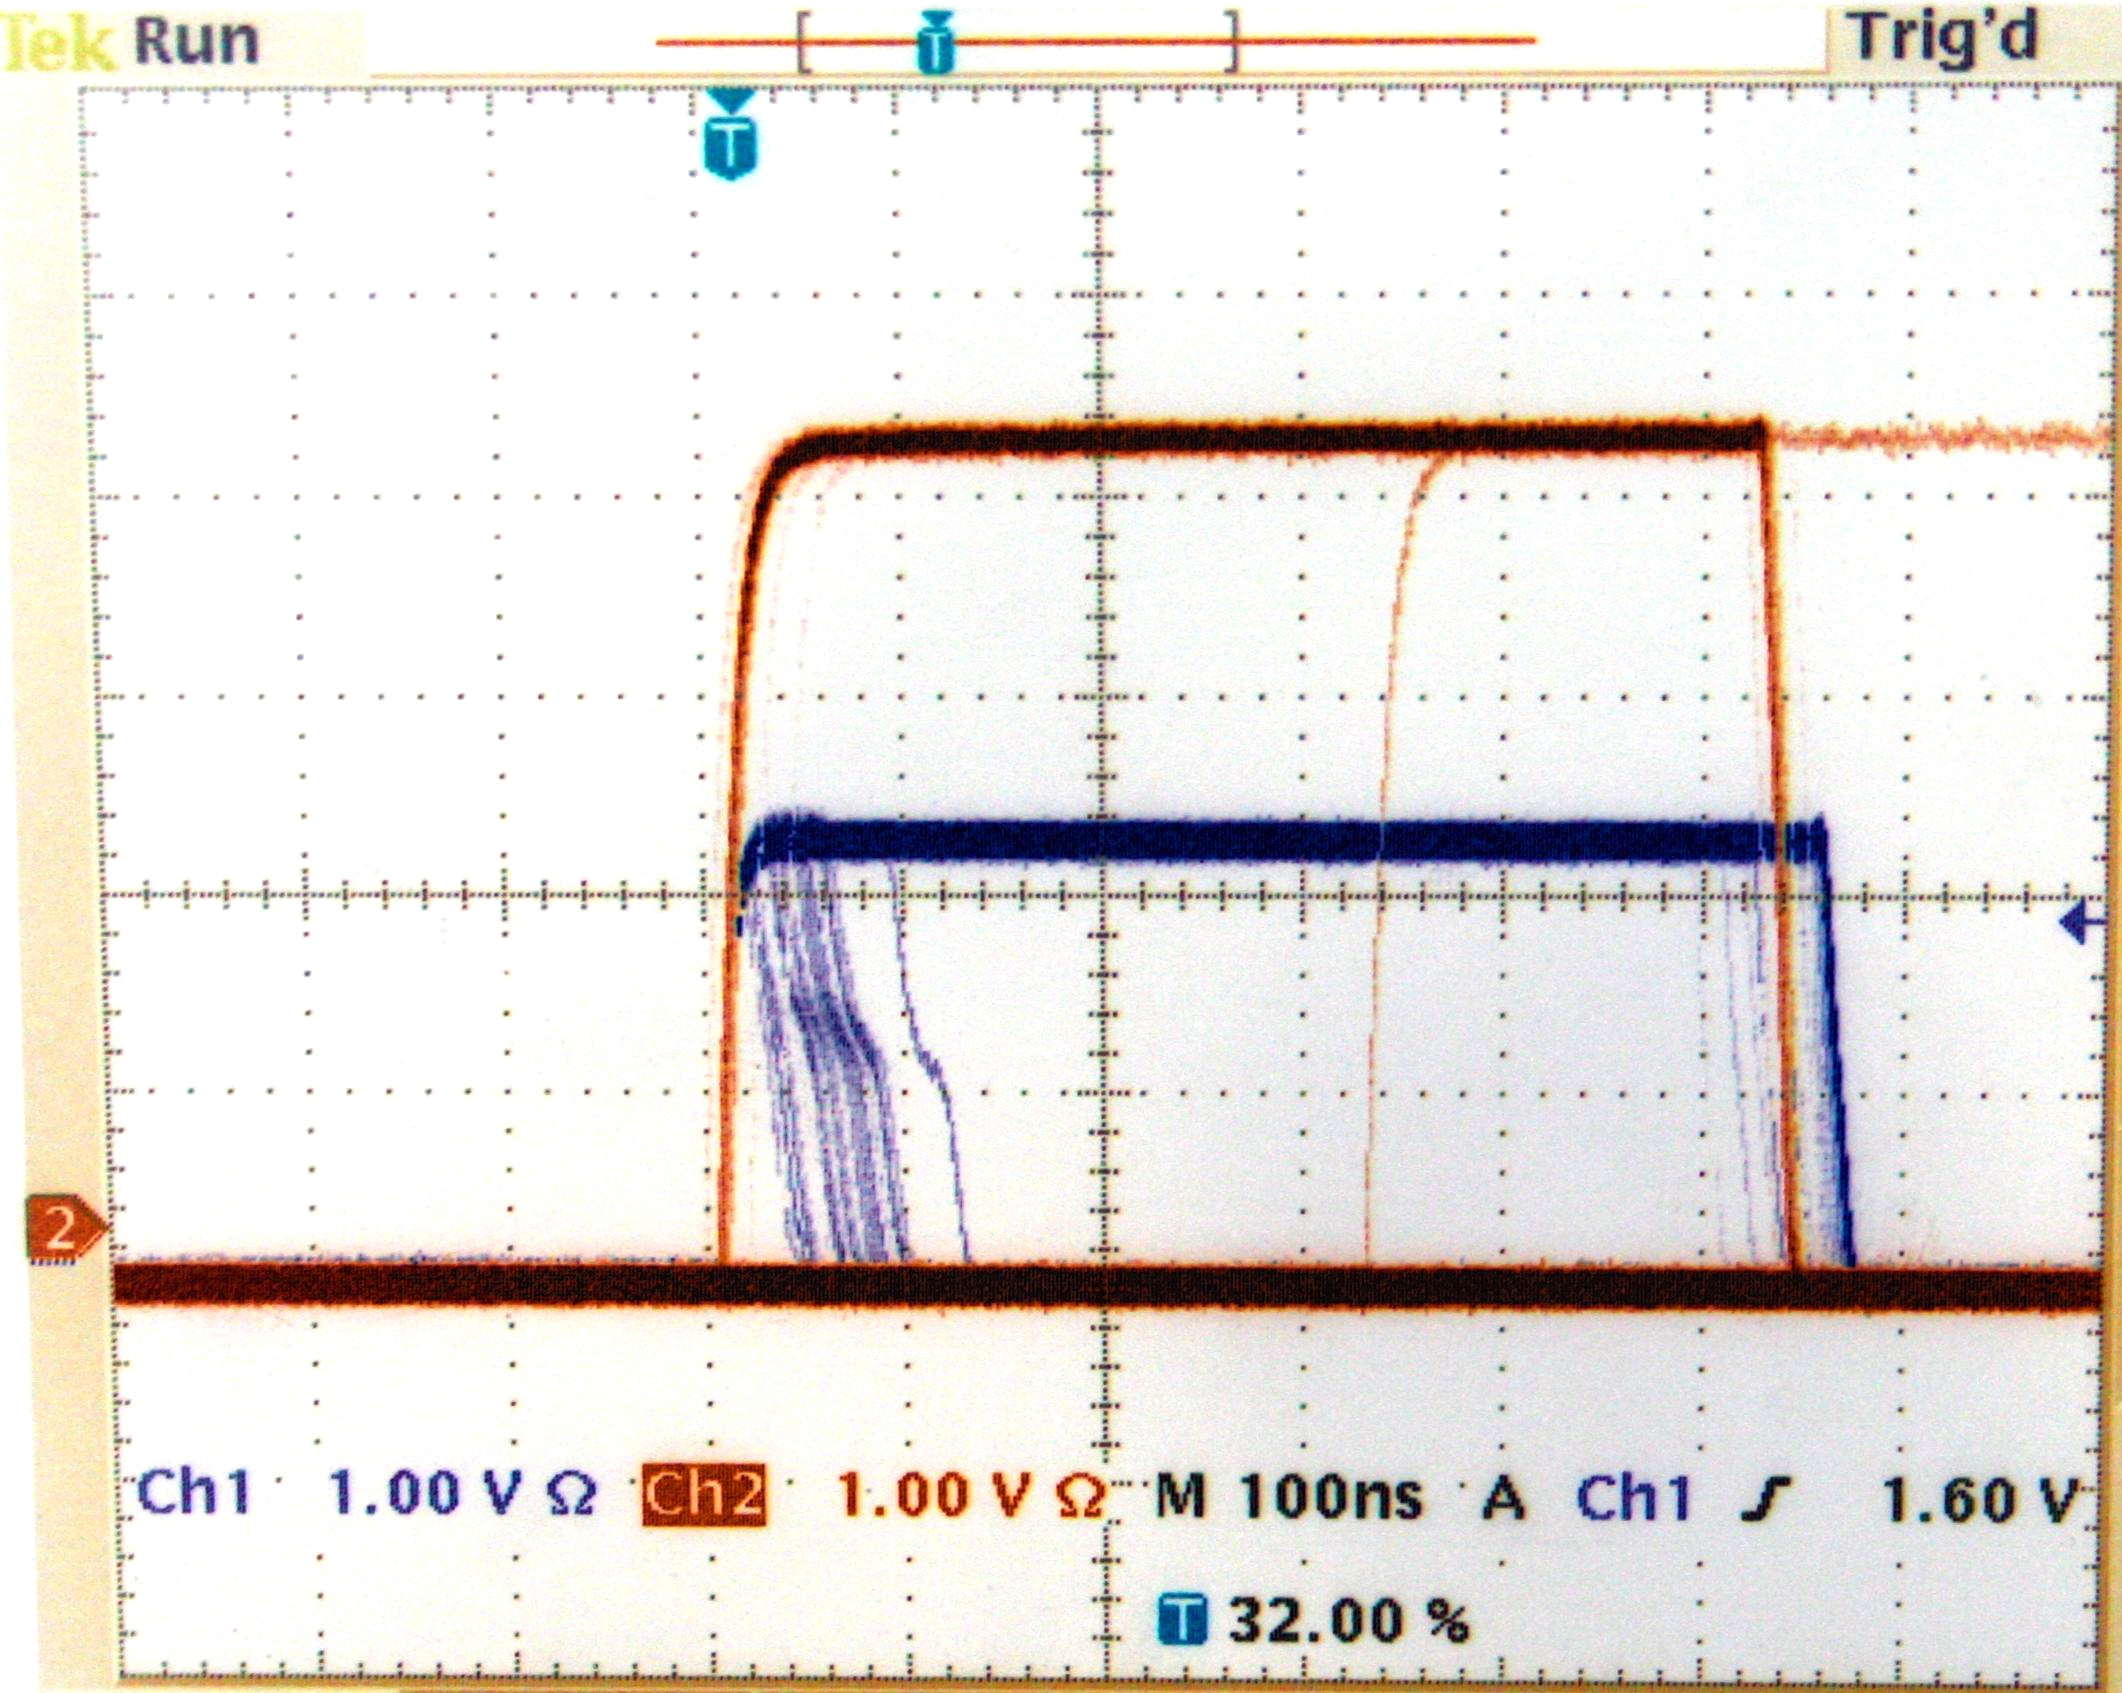
\includegraphics[height=\oscillatorSize\textheight]{br-1-sca-coincidence-511}
\end{frame}

\begin{frame}
    \frametitle{SCA and slow-signal on \SI{511}{\kilo\electronvolt}}

    \centering
    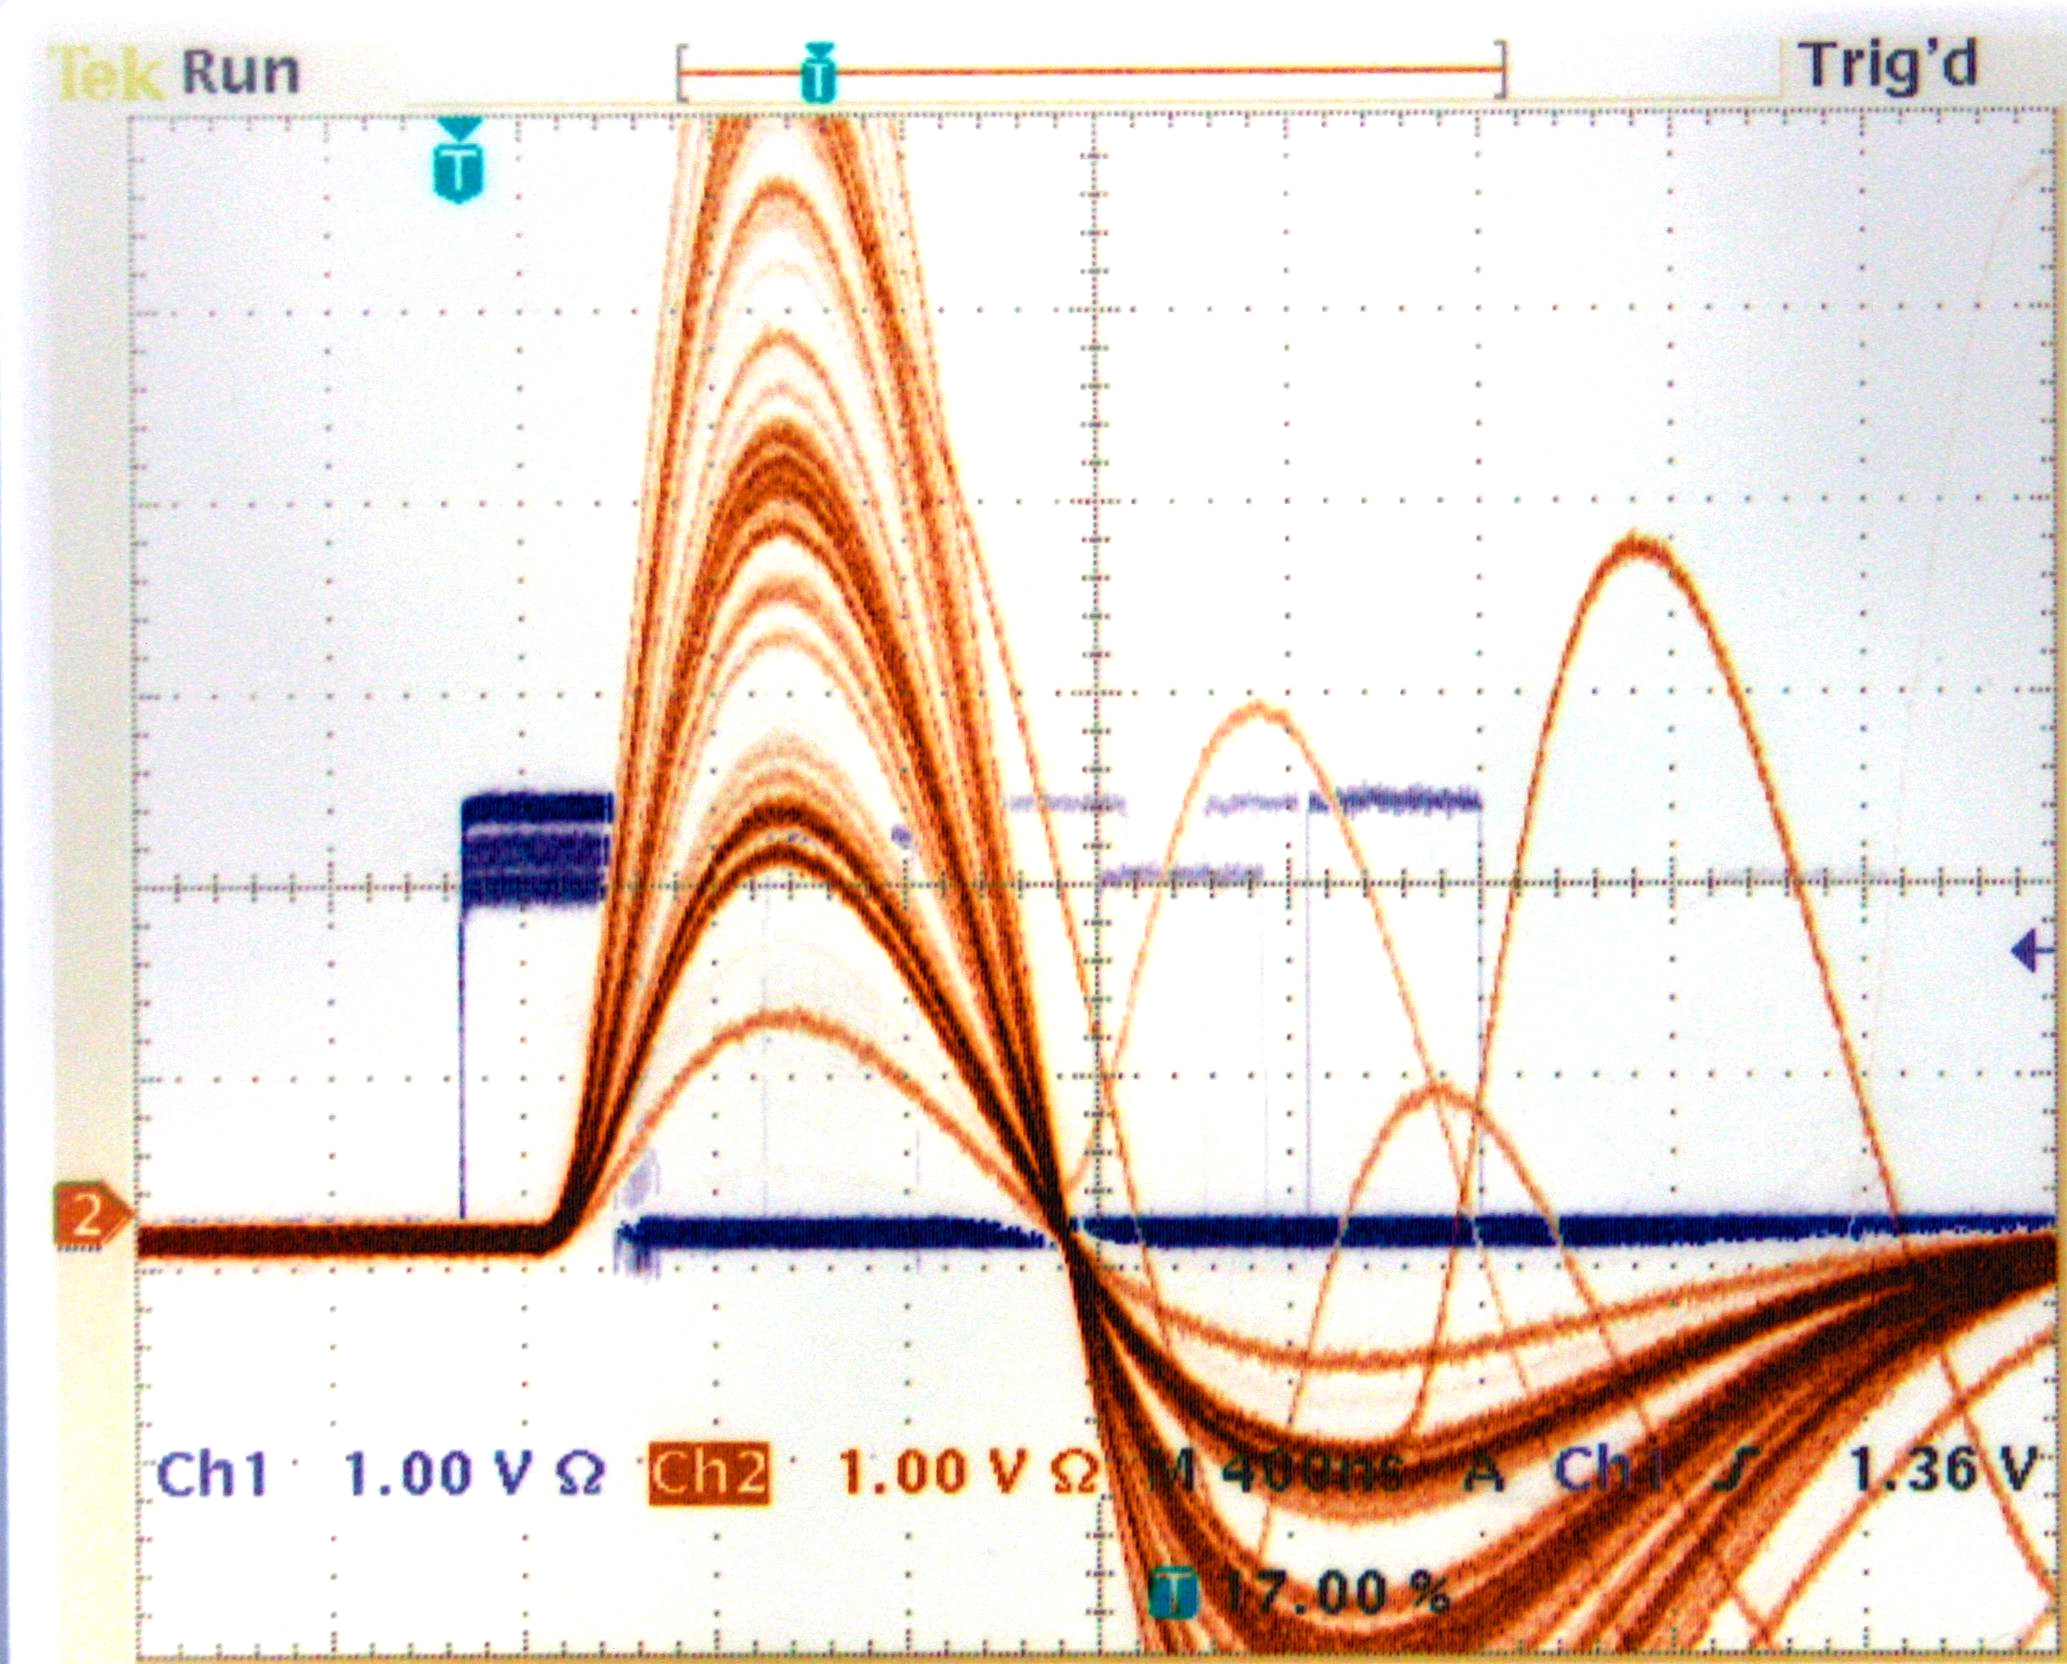
\includegraphics[height=\oscillatorSize\textheight]{br-2-sca-and-slow}
\end{frame}

\subsection{Fast circuit setup}

\begin{frame}
    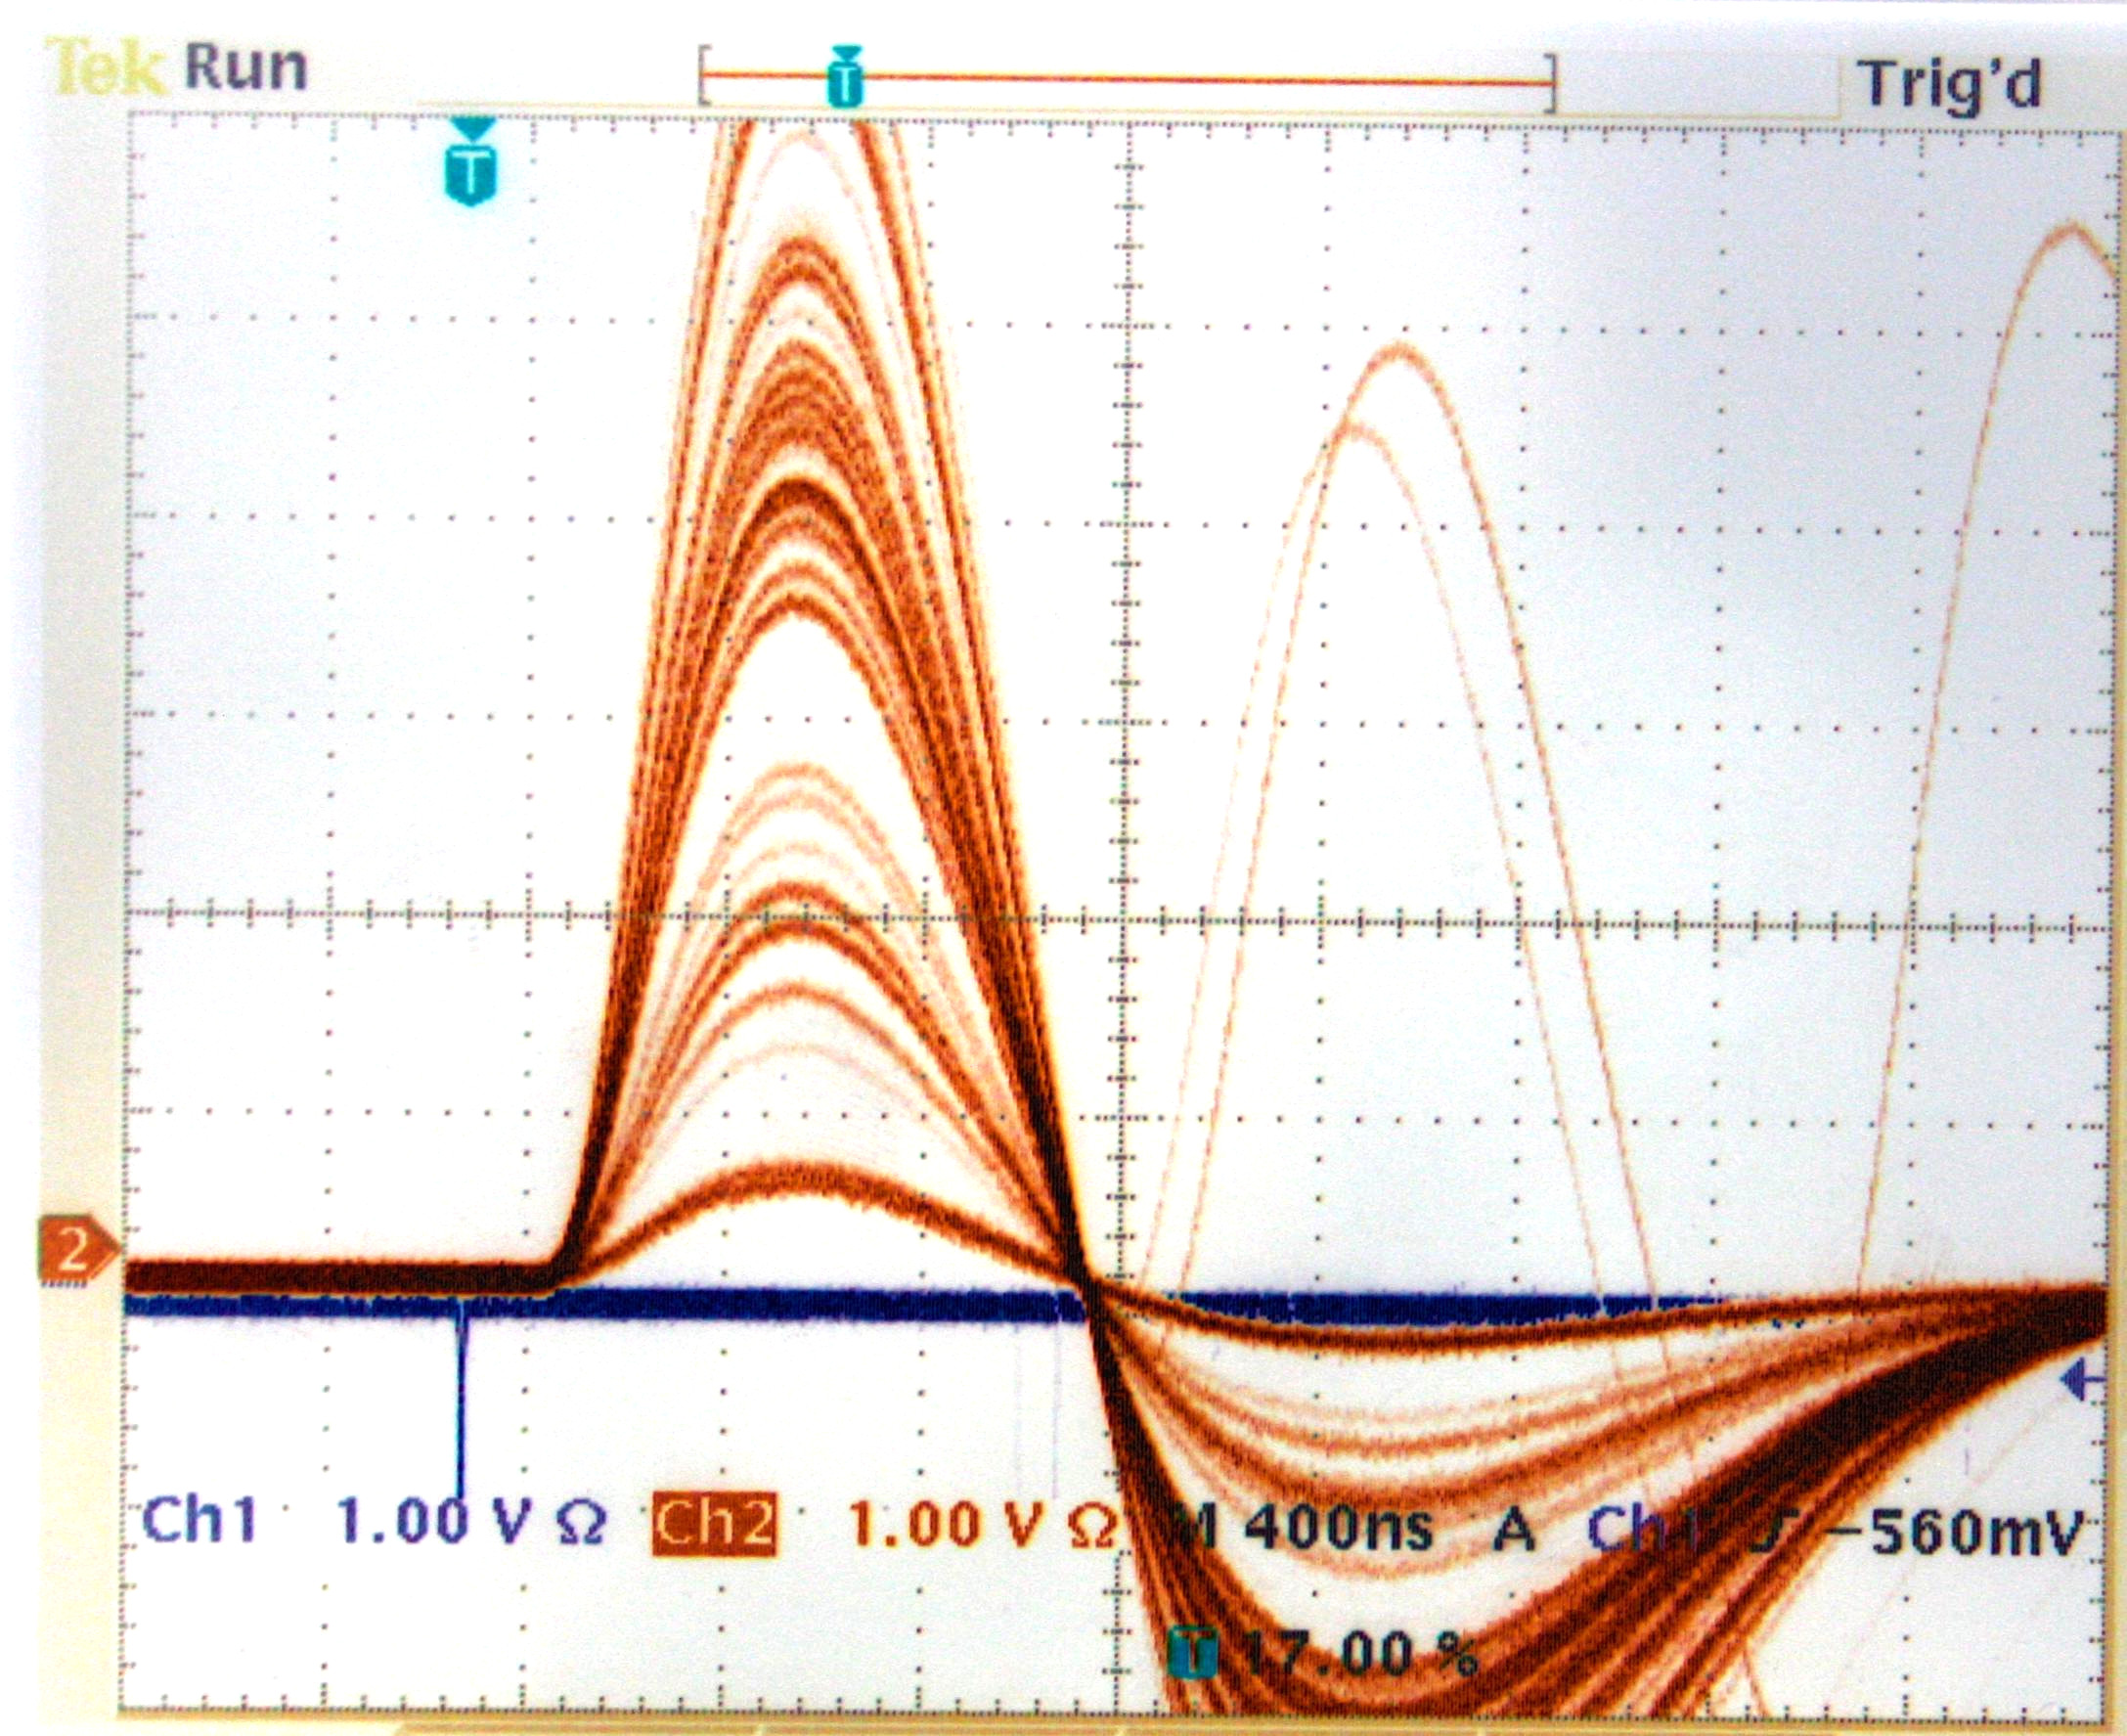
\includegraphics[height=\oscillatorSize\textheight]{br-3-cfd-and-slow}
\end{frame}

\begin{frame}
    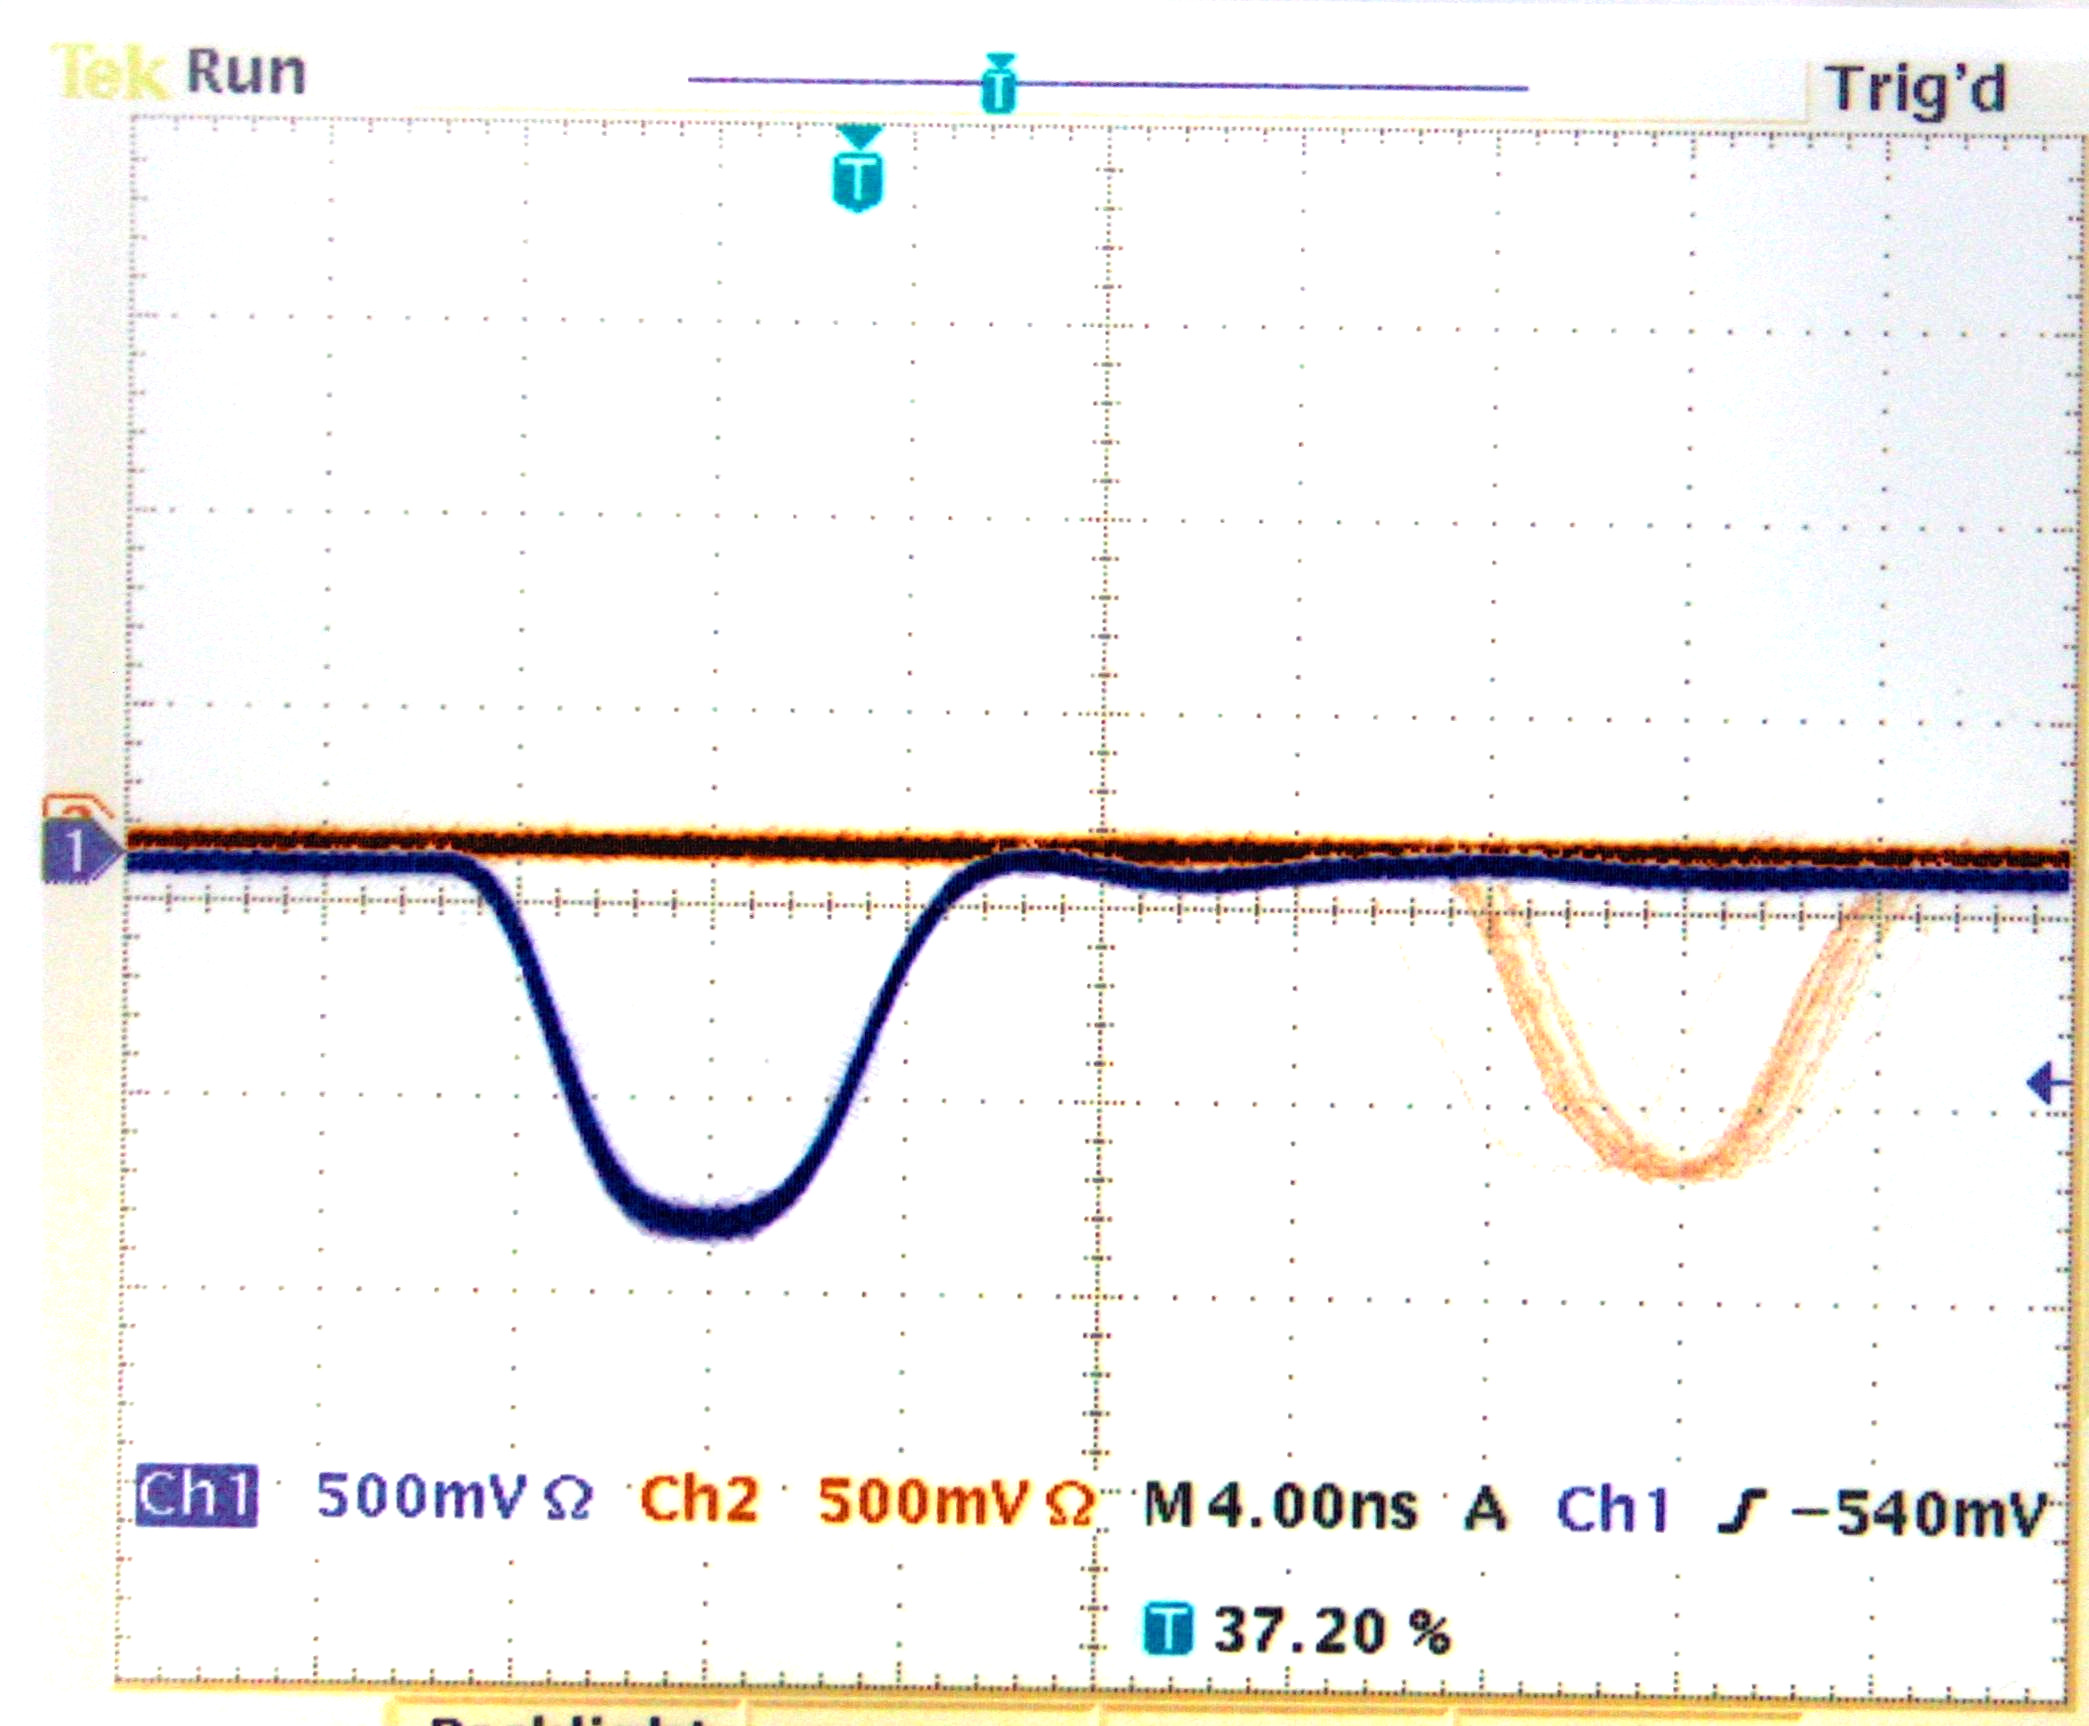
\includegraphics[height=\oscillatorSize\textheight]{br-4-cfd-delay}
\end{frame}

\subsection{Time calibration}

\begin{frame}
    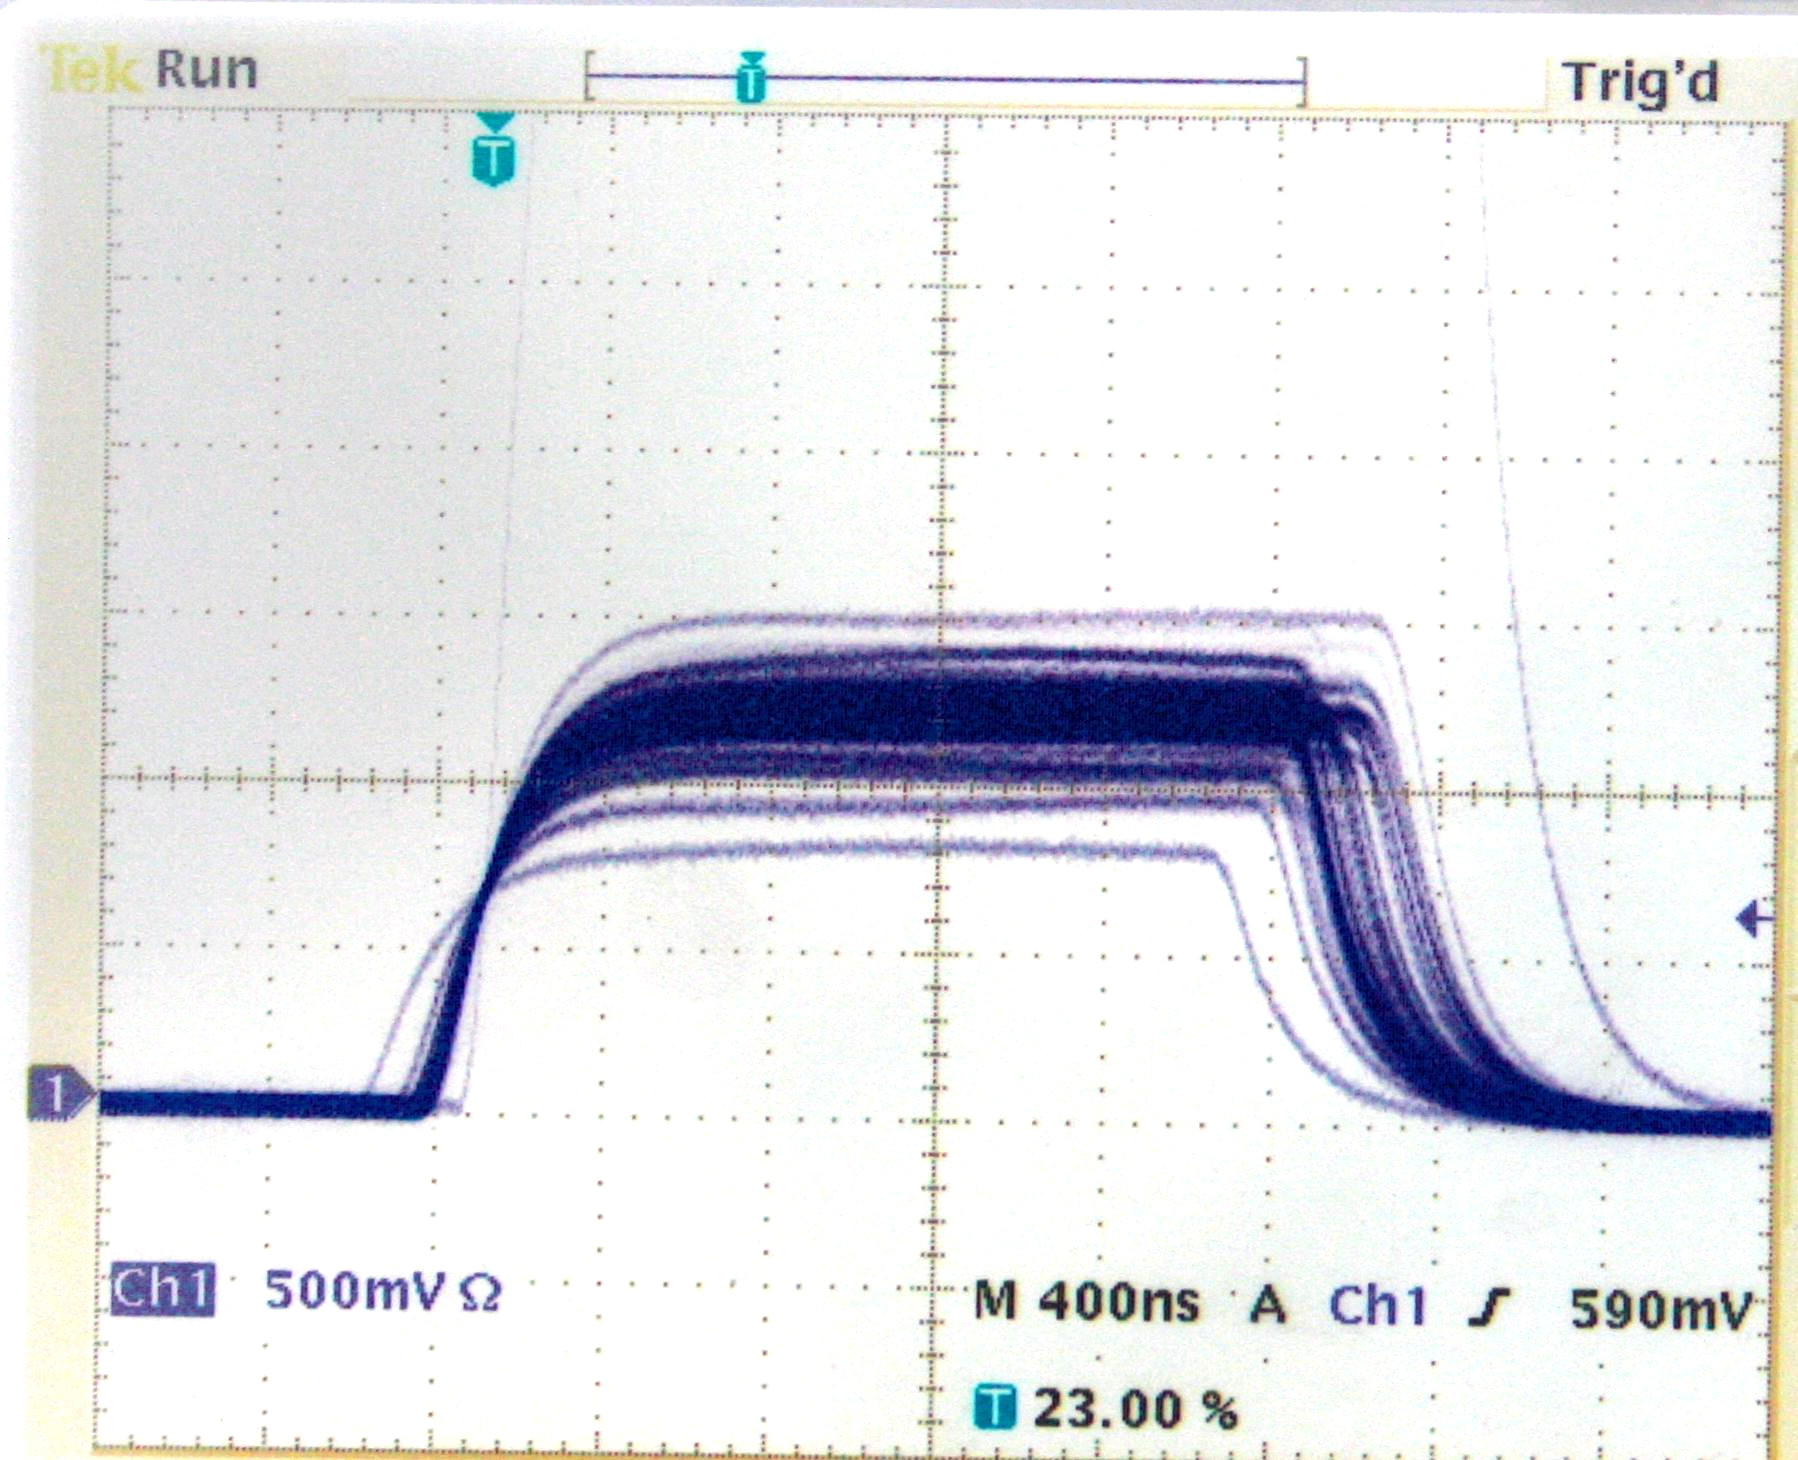
\includegraphics[height=\oscillatorSize\textheight]{br-5-tac-511}
\end{frame}

\begin{frame}
    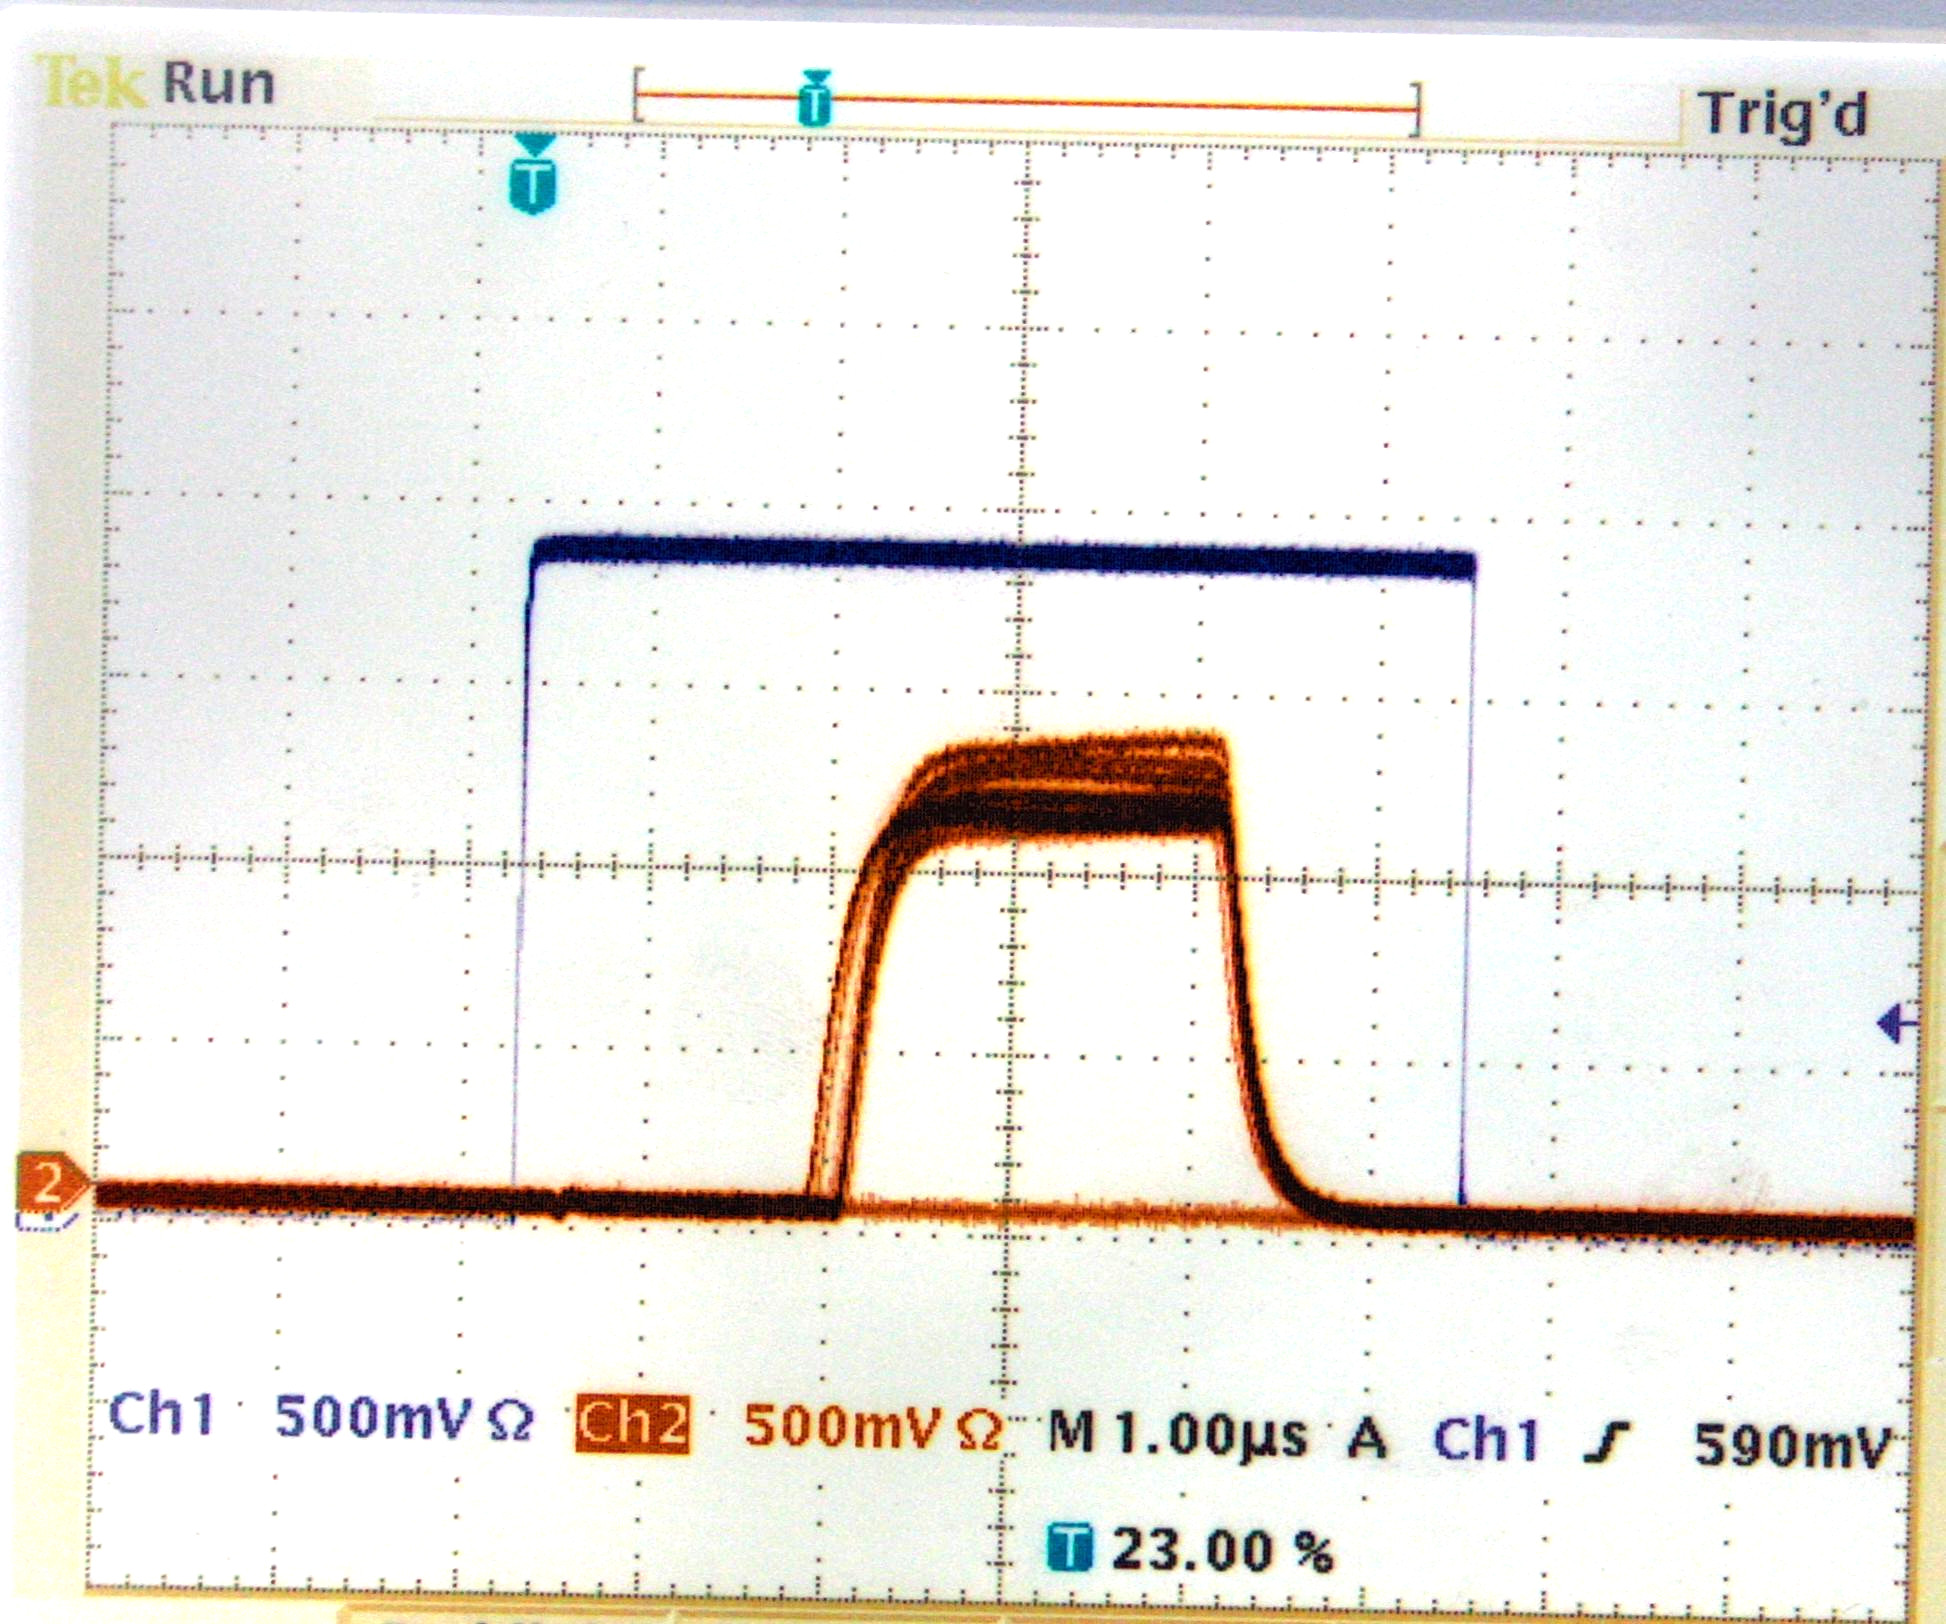
\includegraphics[height=\oscillatorSize\textheight]{br-6-tac-and-coincidence-511}
\end{frame}

\begin{frame}
    \includegraphics{beamer-prompts_short}
\end{frame}

\begin{frame}
    \includegraphics{beamer-prompts_long}
\end{frame}

\begin{frame}
    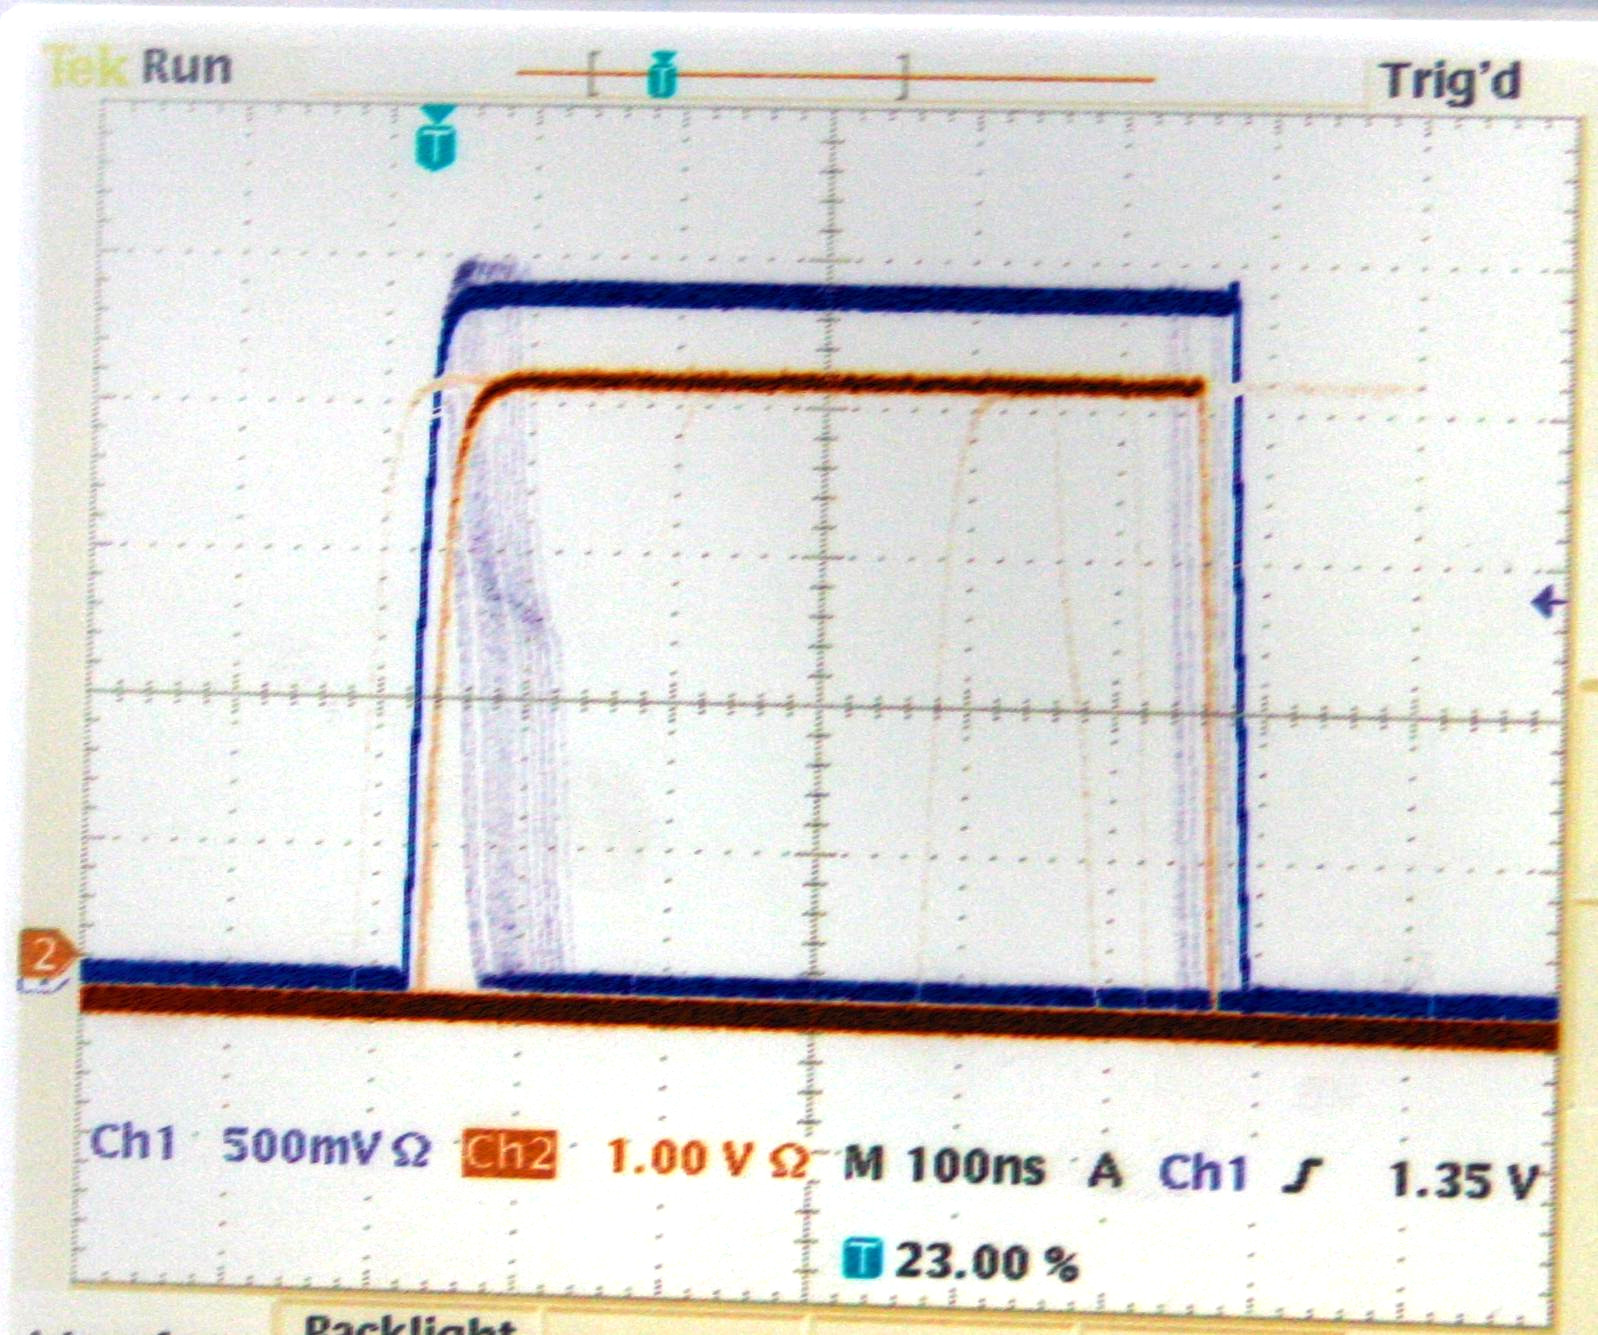
\includegraphics[height=\oscillatorSize\textheight]{br-7-sca-coincidence-1275}
\end{frame}

\begin{frame}
    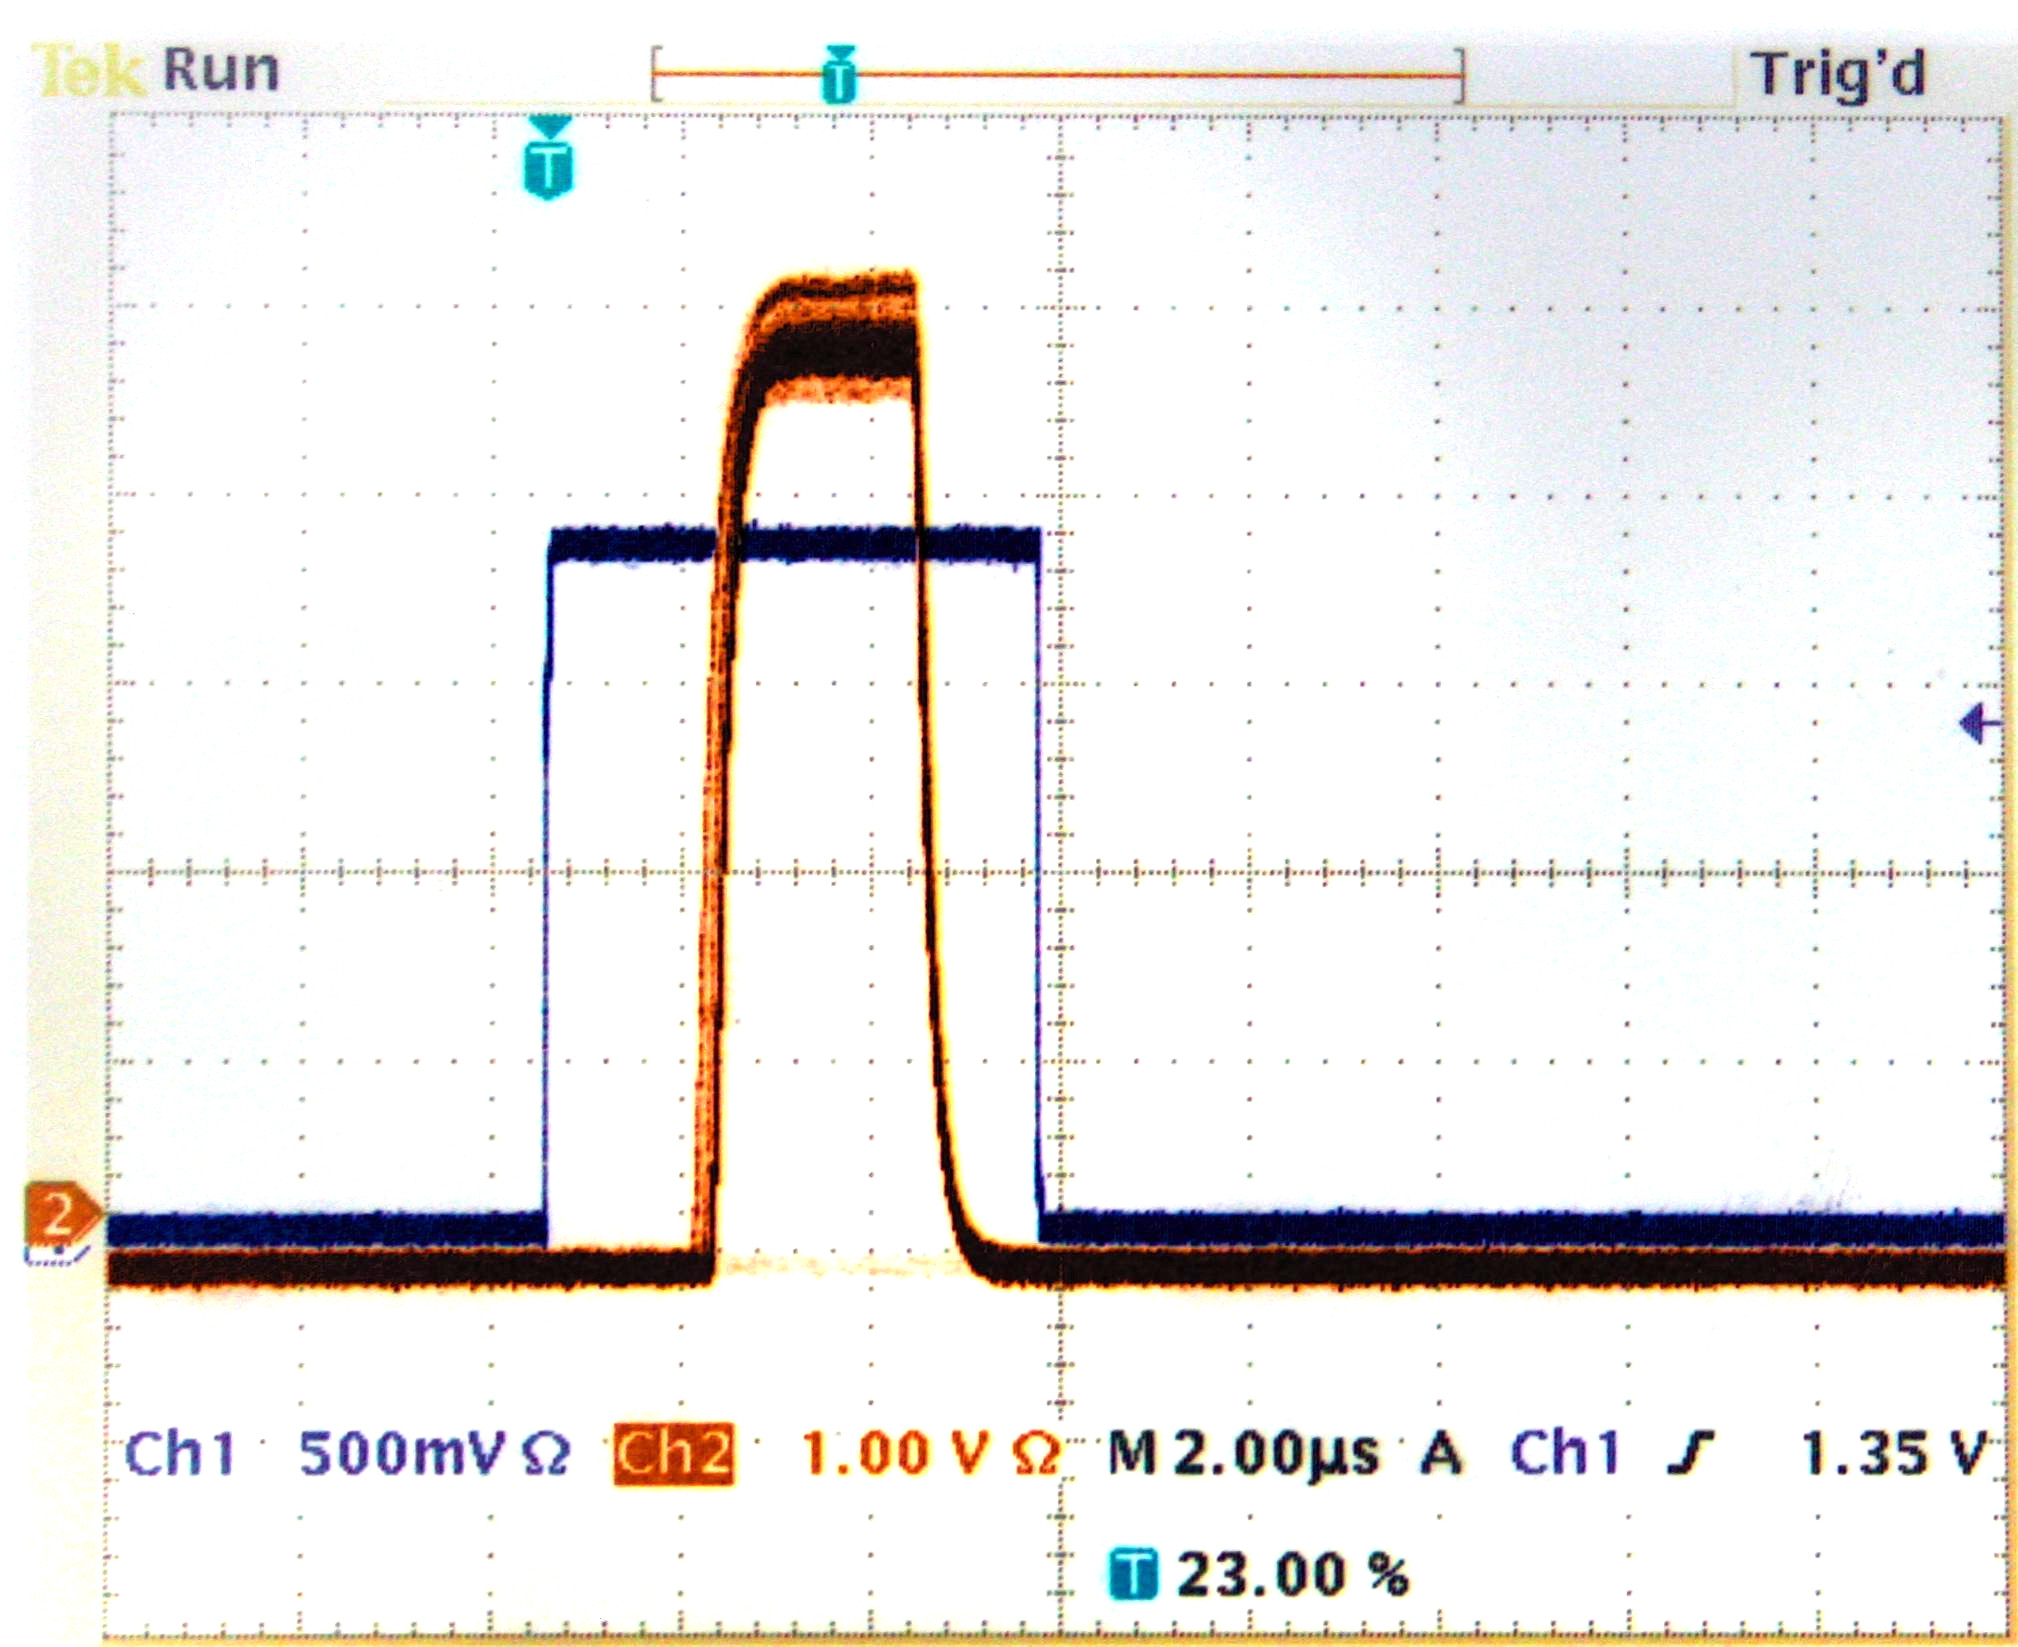
\includegraphics[height=\oscillatorSize\textheight]{br-8-tac-and-coincidence-1275}
\end{frame}

\subsection{Lifetime measurement}

\begin{frame}
    \frametitle{Lifetime at room temperature}

    \centering
    \includegraphics{beamer-lifetime-295K}
\end{frame}

\section{Analysis}

\transition{Analysis}{crunch1}

\subsection{Time gauge}

\begin{frame}
    \frametitle{Conversion}

    We need to convert MCA channels into durations.
\end{frame}

\begin{frame}
    \frametitle{Recall the prompt curves}

    \centering
    \includegraphics{beamer-prompts_short}
\end{frame}

\begin{frame}
    \frametitle{Channel -- delay relation}

    \centering
    \includegraphics{beamer-time_gauge}
\end{frame}

\begin{frame}
    \frametitle{Channel -- delay relation}

    A linear fit (with Jackknife) gives
    \SI{<< time_gauge_slope >>}{\milli\second} per channel
\end{frame}


\begin{frame}
    \frametitle{Time resolution}

    \centering
    \includegraphics{beamer-prompts_long}
\end{frame}

\begin{frame}
    \frametitle{Time resolution}

    Resolution of \SI{<< time_resolution >>}{\nano\second}
\end{frame}

\subsection{Lifetimes}

\begin{frame}
    \frametitle{Now to the lifetime spectra}
    
    \centering
    \includegraphics{beamer-lifetime-295K}
\end{frame}

\begin{frame}
    \frametitle{Lifetime model}

    Model is a combination of
    \begin{itemize}
        \item Resolution function (width, central value)
        \item Short lived component (lifetime, amplitude)
        \item Long lived component (lifetime, amplitude)
        \item Constant offset
    \end{itemize}
\end{frame}

\begin{frame}
    \frametitle{Relative intensities}

    \centering
    \includegraphics{beamer-intensities}
\end{frame}

\begin{frame}
    \frametitle{Extracted lifetimes}

    \centering
    \includegraphics{beamer-taus}
\end{frame}

\subsection{Vacancy formation enthalpy}

\begin{frame}
    \frametitle{Mean lifetime / S-curve}

    \centering
    \includegraphics{beamer-s_curve}
\end{frame}

\begin{frame}
    \frametitle{Arrhenius plot}

    \centering
    \includegraphics{beamer-arrhenius}
\end{frame}

\begin{frame}
    \frametitle{Result}

    Our result:
    \[
        H_\text t = \SI{<< Ht_eV >>}{\electronvolt}
    \]

    \pause

    Literature \parencite[(7a)]{Weiler/Vacancy_formation}:
    \[
        H_\text t = \SI{0.54 +- 0.03}{\electronvolt}
    \]

    \alert{Does not match at all!}
\end{frame}

\subsection{Acrylic glass}

\begin{frame}
    \frametitle{Lifetime in acrylic glass}

    \centering
    \includegraphics{beamer-acrylic}
\end{frame}

\begin{frame}
    \frametitle{Lifetime in acrylic glass (zoom)}

    \centering
    \includegraphics{beamer-acrylic-zoom}
\end{frame}

\begin{frame}
    \frametitle{Fit results}

    Preliminary fit:
    \[
        \tau_0 = \SI{<< acryl_tau_0_lin >>}{\nano\second}
        \qquad
        \tau_\text t = \SI{<< acryl_tau_t_lin >>}{\nano\second}
    \]

    Complete fit:
        \begin{gather*}
            \tau_0 = \SI{<< acryl_tau_0 >>}{\nano\second}
            \qquad
            \tau_\text t = \SI{<< acryl_tau_t >>}{\nano\second} \\
            \tau_\text f = \SI{<< acryl_tau_f >>}{\nano\second}
            \qquad
            \bar\tau = \SI{<< acryl_tau_bar >>}{\nano\second}
        \end{gather*}
\end{frame}

% \includegraphics{lifetime-<< temp >>K}

\begin{frame}
    \frametitle{References}

    \printbibliography
\end{frame}

\end{document}

% vim: spell spelllang=en_us
